\pagebreak
\section{Steering test} %\label{put a label here and uncomment}
\textbf{Name: Group 510}\\
\textbf{Date: 28/10 - 2015}

\subsection{Purpose}
The purpose of the test is to find the needed order of the steering model.

\subsection{Theory}


What is the input and output of the test?

cirkel figure

cirkel figure description (avoiding measuring angle to improve accdapowjda.)

(The hall sensor is not used for putting points around the arc, since just taking manual point will be faster, furthermore we will not use it to get the angle, because it will be to difficult to get an exact angle)

equations from the cirkel:

radius

angular velocity

\subsection{Setup}
\begin{figure}[H]
  \centering
	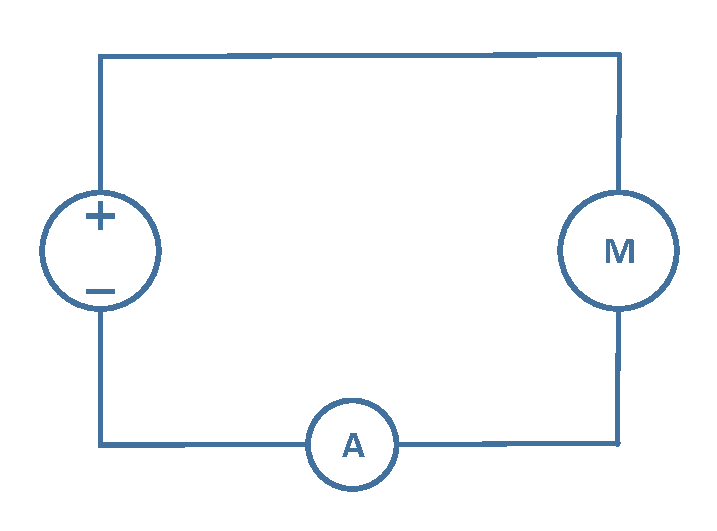
\includegraphics[scale=0.5]{figures/FrictionTest.pdf}
	\caption{A diagram of the test setup}
\end{figure}

\subsection{List of Equipment}

\begin{table}[H]
\begin{tabular}{|l|l|p{4cm}|}
\hline%------------------------------------------------------------------------------------
  \textbf{Instrument}                       &  \textbf{AAU-no.}  &  \textbf{Type}         \\
\hline%------------------------------------------------------------------------------------
  Multimeter                                &  60764             &  Fluke 189 true RMS    \\
\hline%------------------------------------------------------------------------------------
  Power Supply ($0 - 32$ V) ($0 - 10$ A)    &  77075             &  Ea - ps 7032 - 100    \\
\hline%------------------------------------------------------------------------------------
  Treadmill                                 &  75483             &  Rodby                 \\
\hline%------------------------------------------------------------------------------------
\end{tabular}
\end{table}

\subsection{Procedure}

\begin{enumerate}
  \item C
  \item P
  \item S
  \item A
  \item C
  \item R
  \item R
\end{enumerate}

\subsection{Results}


